\section{Results} \label{Results}

\subsection{Main Results}

Figure \ref{ResultsPlot} shows estimated dynamic treatment effects and 95\% confidence intervals for all students and the four subgroups of interest. 

\begin{figure}[!h]
	\centering
	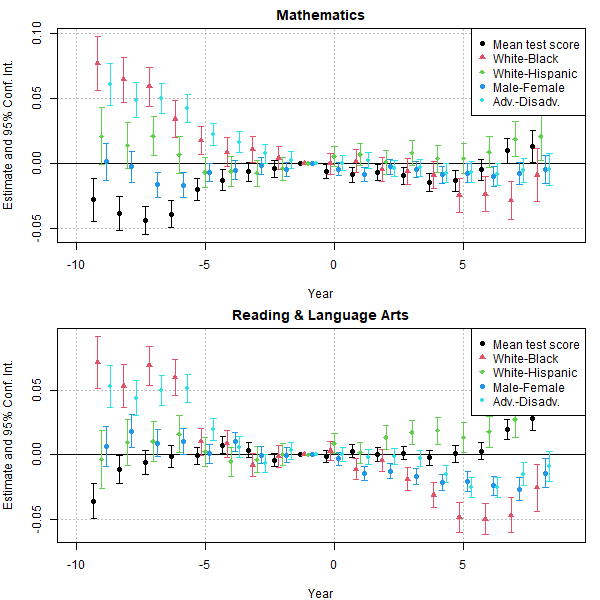
\includegraphics[scale=1]{"../Code & Data/ResultsPlot.pdf"}
	\caption{Dynamic Treatment effects in relative time: FEMA disaster data}
	\label{ResultsPlot}
\end{figure}


For the period of treatment there is a significant\footnote{Significant is used here in the sense that a confidence interval with nominal coverage of 95\% does not include zero, that is a corresponding t-test would reject the null hypothesis of a zero effect at the 5\% level.} effect of natural disasters on the performance in mathematics. The effect size is between just above zero and -0.01 standard deviations. Also, one year after the disaster there is an even larger significant decrease in test scores. For all subsequent periods the effect is not significant. There are some point estimates well below zero, but the uncertainty around those is relatively large. For performance in RLA, there are no significant effects.

Note that the number of observed units decreases with the distance in time from treatment. The reason for this is that in order to experience eight treated years, the county has to experience its first disaster very early. Similarly, it has to receive treatment very late to experience more than five years before treatment. As a result, the uncertainty increases with the distance in time from treatment.

For the subgroups we find some surprising results. Black students seem to perform better in RLA in the medium term after a disaster. That is, there are significantly positive results one to seven years after treatment. The effect sizes are substantial: Seven years after treatment the increase in RLA performance goes up to 0.1 standard deviations. In other words, the average black student sees an increase in performance of up to 0.1 standard deviations of the national reference cohort. Also, hispanic students score significantly lower in mathematics in the year following a disaster.

Positive effects of disasters on performance are not unheard of in the literature. In fact, this is somewhat consistent with the findings by \cite{Sacerdote_2012}. Many students have to switch schools and some may even benefit from attending a higher quality school after the disaster. Black students may disproportionally attend lower quality schools and are therefore more likely to benefit from having to switch schools. 

Among the subgroubs, we see a few significant pre-treatment estimates. Therefore, the treatment led to a significant difference in average test scores between treatment and control group before the treatment even began. This is likely caused by a violation of one of the two identifiying assumptions: Either the trends in outcomes of treatment and control group are not parallel or treated units anticipated treatment and therefore already saw an effect earlier. Since the latter is rather implausible, we conclude that there might be a violation of the parallel trends assumption. Thus, the affected results have to be interpreted with caution.

Figures \ref{ResultsPlotStorm} shows the same graphs based on the storm treatment. The results look very similar. In the period of the storm there is a significant decrease in mathematics scores of up to -0.015 standard deviations. For the years following treatment there are no significant effects.

For female students there is a significant decrease in both subjects in the period of the storm. For RLA we even find a significantly negative effect one year after the storm. Similarly, economically disadvantaged students perform worse in the period of treatment and in RLA one year after treatment. The effect sizes range from barely above zero up to -0.015 or even -0.02 standard deviations. For black and hispanic students we do not find any significant effects of the storm treatment.

\begin{figure}[!h]
	\centering
	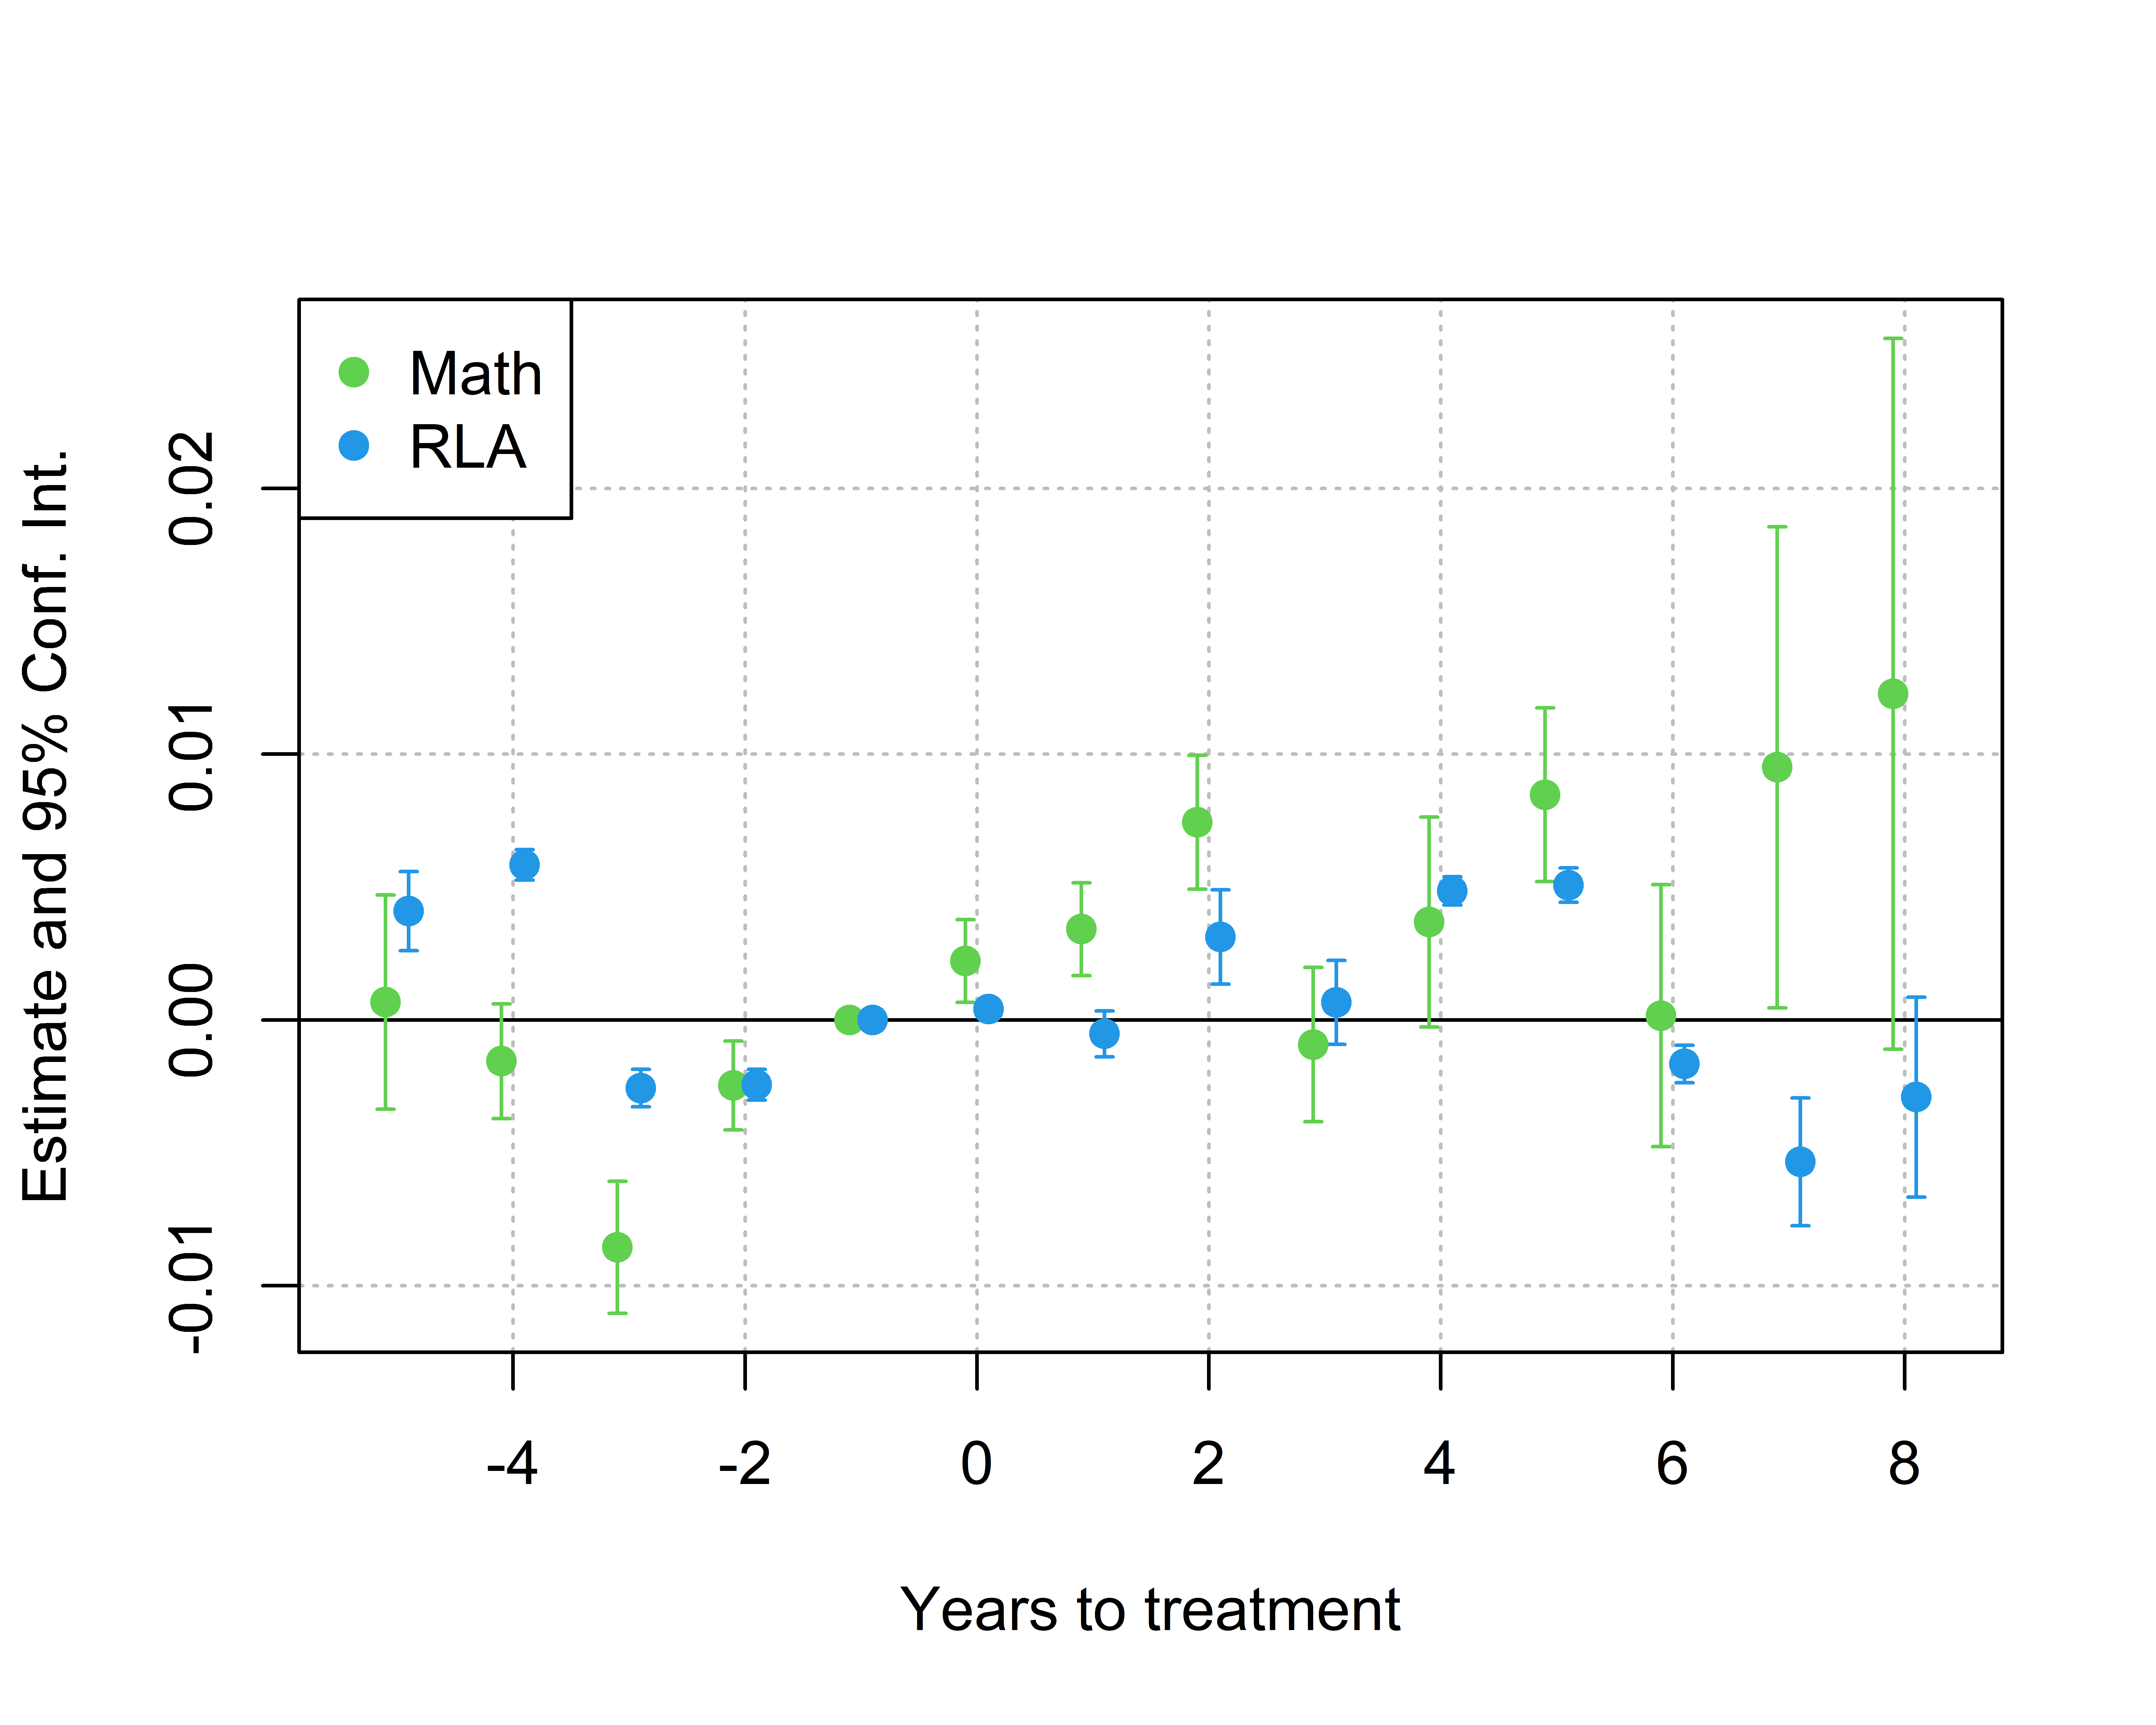
\includegraphics[scale=1]{"../Code & Data/ResultsPlotStorm.pdf"}
	\caption{Dynamic Treatment effects in relative time: NWS storm data}
	\label{ResultsPlotStorm}
\end{figure}


\subsection{Heat Results}

Table \ref{tab:HeatResults} provides the estimation results for the heat models. Rows 1 and 2 show the estimated coefficients and standard errors for the maximum temperature variable for mathematics and RLA respectively.

At a 0.05 significance level the estimate is not significant for the entire student population in both mathematics and RLA. However, we find significant results for the subgroups with point estimates between $-0.001$ and $-0.002$. This implies, the effect of an on average 5°C hotter school year is comparable to the average effect of a natural disaster in the same year.


\begin{tabular}{lllllll}
\toprule
  & Overall & White & Black & Hispanic & Female & Econ. Disadv.\\
\midrule
Max. Temp. (Math) & $-0.0007$ & $-0.0002$ & $-0.0006$ & $-0.0021^{***}$ & $-0.001^{***}$ & $-0.0011^{***}$\\
 & $(0.0003)$ & $(0.0004)$ & $(0.0008)$ & $(0.0006)$ & $(0.0004)$ & $(0.0004)$\\
\addlinespace
Max. Temp. (RLA) & $-0.0001$ & $0.0005$ & $-0.0015^{***}$ & $-0.0011^{***}$ & $-0.0002$ & $-0.0004$\\
 & $(0.0003)$ & $(0.0003)$ & $(0.0007)$ & $(0.0006)$ & $(0.0003)$ & $(0.0003)$\\
\addlinespace
Days ab. 30 (Math) & $-0.000169$ & $-0.000111$ & $0.000033$ & $-0.000196$ & $0.000003$ & $0.000003$\\
 & $(0.000089)$ & $(0.000096)$ & $(0.000143)$ & $(0.000136)$ & $(0.000095)$ & $(0.000096)$\\
\addlinespace
Days ab. 30 (RLA) & $-0.000095$ & $-0.000178^{***}$ & $-0.00014$ & $-0.000483^{***}$ & $-0.000202^{***}$ & $-0.000027$\\
 & $(0.000071)$ & $(0.000079)$ & $(0.000122)$ & $(0.000117)$ & $(0.000079)$ & $(0.000079)$\\
\addlinespace
\midrule
Mean & -0.042 & 0.107 & -0.483 & -0.281 & 0.025 & -0.284\\
\bottomrule
\end{tabular}


Rows 3 and 4 of Table \ref{tab:HeatResults} show the same results for the number of days above 30°C. Here, we only find a significant effect on hispanic and female students in RLA. For hispanic students the point estimate is $-0.0005$, meaning about 20 additional days above 30°C would be somewhat comparable to the average effect of a natural disaster in the same year.

In total, we only find weak evidence for a negative effect of heat on the achievement in standardized tests. However, it is more pronounced among some subgroups. For hispanic students the estimates indicate significantly negative effects in three out of four specifications with rather large effect sizes. The larger impact on the academic performance of minority students is consistent with other authors' findings \citep[for example][]{Goodman_2020}

One explaining factor could be the presence of air-conditioning. The results in \cite{Goodman_2020} suggest that air conditioning offsets about three quarters of the negative effect of heat exposure. Possibly, counties with higher shares of minority students tend to have a lower presence of air-conditioning in schools. Also, black and hispanic households tend to be poorer on average and may therefore be less likely to have air-conditioning at home. This could explain some of the heterogeneity in the effect of heat.


\subsection{Discussion}

It could be the case that medium- and long-term effects are largely driven by migration. This is a prominent theme in previous studies on disasters and learning \citep{Pane_2008, Sacerdote_2012}. That's why it may be interesting to have a look at the ethnic composition of the counties relative to initial treatment. Figure \ref{EthnicComposition} shows ethnic shares of enrolled students for the treated counties in relative time.

\begin{figure}[!h]
	\centering
	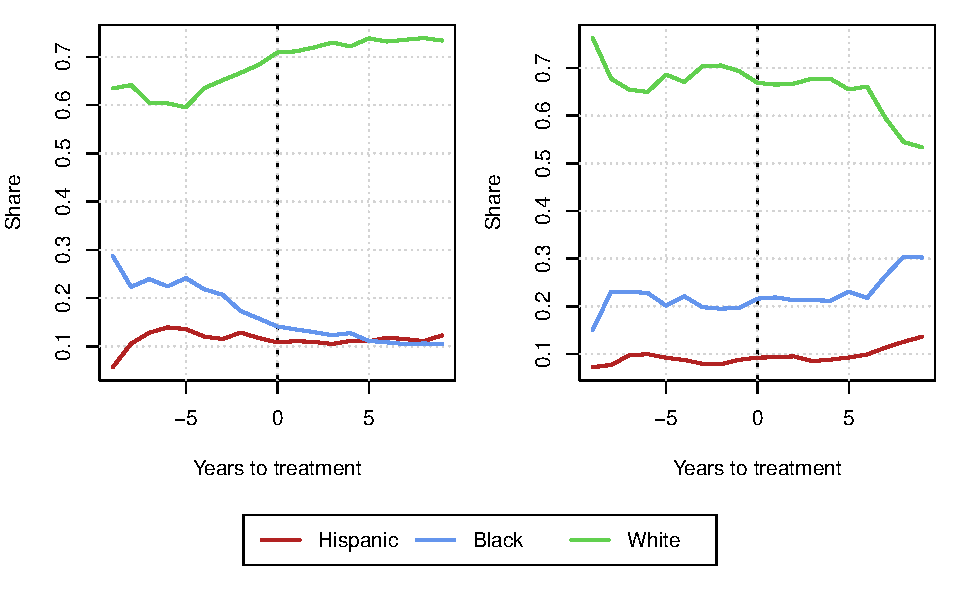
\includegraphics[scale=1]{"../Code & Data/EthnicComposition.pdf"}
	\caption{Aggregated ethnic shares of enrolled students by treatment timing based on FEMA disasters (left) and on NWS storms (right)}
	\label{EthnicComposition}
\end{figure}

In the left panel we see that the share of black students decreases in counties that experienced a disaster. This supports the hypothesis that black students disproportionately switch schools after disasters and may explain the positive long term effect as described above. However, the share of black students already decreases before treatment, so this may not be a causal effect of the disaster.

The same plot based on the NWS storm data shows a different picture. Here, all three shares remain somewhat constant until five years fter treatment. Then the share of black students increases, while the share of white students decreases. This suggests that the migration response to storms may be qualitatively different than the response to other forms of disasters. At least for the storms data this does not seem to be a major driver of the results.

A more in-depth analysis of migration responses to natural disasters and their role in academic achievement is unfortunately not possible with this data. There is some prior research based on individual level data indicating that it does play an important role \citep[for example][]{Sacerdote_2012}. Analyzing migration responses and their link to academic achievement for different types of natural disasters may be a promising area for future research.

For the heat results, we find substantial heterogeneity: Minorities seem to be more prone to adverse effects of heat exposure. The results in \cite{Goodman_2020} indicate that air-conditioning mitigates a large part of the negative effect. Based on that, we speculate that inequality in air-conditioning is the main driver of said heterogeneity, since minority students tend to have less access to air-conditioning. Improving the air-conditioning coverage in more affected schools could be an easy way for policymakers to adress the adverse effects of heat on academic achievement. However, to the best of our knowledge \cite{Goodman_2020} is the only paper to study this relationship. More research on the interconnection between heat, learning, and air-conditioning may be useful to make policy decisions.

Obviously, our results come with limitations. First, the parallel trends assumption may be violated in some subgroups. While a visual inspection of pre-treatment trends does not indicate so, we find significant pre-treatment effects. This is typically a sign for such a violation. In particular, this applies to the results for black, hispanic and economically disadvantaged students based on the FEMA data. Therefore, we have to be more careful when interpreting these results.

Second, the measures of heat exposure used here are based on daily maximum temperature only. However, this likely does not fully capture the physiological impact of heat. Other variables, like humidity or minimum temperatures overnight, can also contribute to the negative effect of heat on learning \citep[for an extensive discussion of heat exposure measurement see][]{Rennie_2021}. It would be desirable to use a more complete measure of heat exposure. The reason why we nevertheless used only the daily maximum temperature is that the data availability for more comprehensive measures is much worse. A reasonable option would be to use gridded satellite data, such as those provided by the Copernicus project\footnote{Available \href{https://climate.copernicus.eu/}{here}}. Unfortunately, these datasets are huge and require much more computational power.


